\documentclass[index]{subfiles}

\begin{document}
\title{Prob \& Stats Exam - Sleep vs. Day}
\author{by Shengdong Li}
\date{2 November 2021}
\maketitle

\section{Source}

My browsing history, journal, and memory

\section{Data Table}

\begin{table}[H]
    \centering
    \caption{The amount of sleep that I've gotten in the past 10 days, in hours}
    \begin{tabularx}{0.20\textwidth}{cX}
        \toprule
        Day \# & Sleep (hrs) \\
        \midrule
        1      & 4.25        \\
        2      & 8.25        \\
        3      & 6.75        \\
        4      & 4.75        \\
        5      & 6.75        \\
        6      & 7.25        \\
        7      & 9.25        \\
        8      & 9.25        \\
        9      & 2.75        \\
        10     & 12.25
    \end{tabularx}
\end{table}

Values for a single day were calculated based on the amount of sleep from noon of the previous day to noon of the current day. For example, day 10 is november 2nd, and its value is the total amount of sleep from noon of november 1st to noon of november 2nd. Day 9 is november 1st, day 8 is october 31st, and so on.

\section{Graph}

\begin{figure}[H]
    \centering
    \textbf{The amount of sleep obtained vs. day number}
    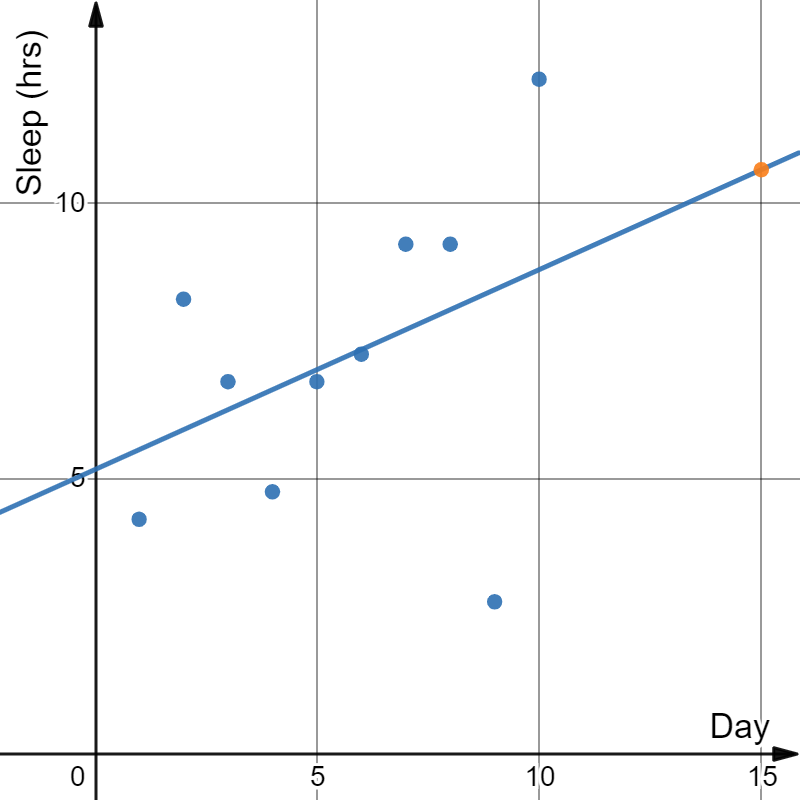
\includegraphics[scale=0.4]{line.png}
    \caption{Graph of line of best fit, along with extrapolated point. Full desmos graph \href{https://www.desmos.com/calculator/iiuzxsqtsf}{here}}
\end{figure}
\begin{align*}
    \intertext{The line of best fit was found to be}
    \Aboxed{y & =0.363636x+5.15}
    \intertext{and the correlation coefficient}
    \Aboxed{r & =0.3951}
    \intertext{With this line of best fit, we can predict the amount of sleep that I'd get on day 15.}
    y         & =0.363636x+5.15               \\
              & =0.363636\left(15\right)+5.15 \\
              & =10.60454                     \\
              & \approx\boxed{10.6}
\end{align*}

\section{Explanation of Correlation Coefficient}

The correlation coefficient is calculated by basically finding the average \(Z\) score for each data point. We know that the \(Z\) score is calculated via
\begin{equation*}
    Z=\frac{x-\mu}{\sigma}
\end{equation*}
which is basically a fractional value of number of standard deviations away from the mean.

An \(r\) value closer to \(1\) for a positively sloped function describes a strong relationship between the line of best fit and the data, and an \(r\) value closer to \(-1\) for a negatively sloped function is also a strong relationship.

In the context of this specific data point, it describes the correlation relationship between the day number and amount of sleep. But because the correlation coefficient is only around \(0.3951\), it means that the data points deviate greatly from the line of best fit, and so the data isn't very reliable at all. In other words, the amount of sleep that I get each night does not have a strong relationship with the general slope of the line of best fit.

\section{Meaning of Slope}

The slope of the line of best fit describes the \(\frac{hours\ of\  sleep}{day}\), or the general trend of change in sleep over time for me. Because the slope is a positive \(0.364\), it means that from the line of best fit, as the days go on I should be getting more and more sleep everyday, gaining approximately \(0.364\) hours of sleep per day. However, because the \(r\) value is so low, the value of this slope should not be trusted.

\end{document}
